% Options for packages loaded elsewhere
\PassOptionsToPackage{unicode}{hyperref}
\PassOptionsToPackage{hyphens}{url}
\PassOptionsToPackage{dvipsnames,svgnames,x11names}{xcolor}
%
\documentclass[
  10pt,
  letterpaper]{article}

\usepackage{amsmath,amssymb}
\usepackage{lmodern}
\usepackage{iftex}
\ifPDFTeX
  \usepackage[T1]{fontenc}
  \usepackage[utf8]{inputenc}
  \usepackage{textcomp} % provide euro and other symbols
\else % if luatex or xetex
  \usepackage{unicode-math}
  \defaultfontfeatures{Scale=MatchLowercase}
  \defaultfontfeatures[\rmfamily]{Ligatures=TeX,Scale=1}
  \setmainfont[]{Charis SIL}
  \setmathfont[]{Monaco}
\fi
% Use upquote if available, for straight quotes in verbatim environments
\IfFileExists{upquote.sty}{\usepackage{upquote}}{}
\IfFileExists{microtype.sty}{% use microtype if available
  \usepackage[]{microtype}
  \UseMicrotypeSet[protrusion]{basicmath} % disable protrusion for tt fonts
}{}
\makeatletter
\@ifundefined{KOMAClassName}{% if non-KOMA class
  \IfFileExists{parskip.sty}{%
    \usepackage{parskip}
  }{% else
    \setlength{\parindent}{0pt}
    \setlength{\parskip}{6pt plus 2pt minus 1pt}}
}{% if KOMA class
  \KOMAoptions{parskip=half}}
\makeatother
\usepackage{xcolor}
\usepackage[margin = 1in]{geometry}
\setlength{\emergencystretch}{3em} % prevent overfull lines
\setcounter{secnumdepth}{-\maxdimen} % remove section numbering
% Make \paragraph and \subparagraph free-standing
\ifx\paragraph\undefined\else
  \let\oldparagraph\paragraph
  \renewcommand{\paragraph}[1]{\oldparagraph{#1}\mbox{}}
\fi
\ifx\subparagraph\undefined\else
  \let\oldsubparagraph\subparagraph
  \renewcommand{\subparagraph}[1]{\oldsubparagraph{#1}\mbox{}}
\fi

\usepackage{color}
\usepackage{fancyvrb}
\newcommand{\VerbBar}{|}
\newcommand{\VERB}{\Verb[commandchars=\\\{\}]}
\DefineVerbatimEnvironment{Highlighting}{Verbatim}{commandchars=\\\{\}}
% Add ',fontsize=\small' for more characters per line
\usepackage{framed}
\definecolor{shadecolor}{RGB}{241,243,245}
\newenvironment{Shaded}{\begin{snugshade}}{\end{snugshade}}
\newcommand{\AlertTok}[1]{\textcolor[rgb]{0.68,0.00,0.00}{#1}}
\newcommand{\AnnotationTok}[1]{\textcolor[rgb]{0.37,0.37,0.37}{#1}}
\newcommand{\AttributeTok}[1]{\textcolor[rgb]{0.40,0.45,0.13}{#1}}
\newcommand{\BaseNTok}[1]{\textcolor[rgb]{0.68,0.00,0.00}{#1}}
\newcommand{\BuiltInTok}[1]{\textcolor[rgb]{0.00,0.23,0.31}{#1}}
\newcommand{\CharTok}[1]{\textcolor[rgb]{0.13,0.47,0.30}{#1}}
\newcommand{\CommentTok}[1]{\textcolor[rgb]{0.37,0.37,0.37}{#1}}
\newcommand{\CommentVarTok}[1]{\textcolor[rgb]{0.37,0.37,0.37}{\textit{#1}}}
\newcommand{\ConstantTok}[1]{\textcolor[rgb]{0.56,0.35,0.01}{#1}}
\newcommand{\ControlFlowTok}[1]{\textcolor[rgb]{0.00,0.23,0.31}{#1}}
\newcommand{\DataTypeTok}[1]{\textcolor[rgb]{0.68,0.00,0.00}{#1}}
\newcommand{\DecValTok}[1]{\textcolor[rgb]{0.68,0.00,0.00}{#1}}
\newcommand{\DocumentationTok}[1]{\textcolor[rgb]{0.37,0.37,0.37}{\textit{#1}}}
\newcommand{\ErrorTok}[1]{\textcolor[rgb]{0.68,0.00,0.00}{#1}}
\newcommand{\ExtensionTok}[1]{\textcolor[rgb]{0.00,0.23,0.31}{#1}}
\newcommand{\FloatTok}[1]{\textcolor[rgb]{0.68,0.00,0.00}{#1}}
\newcommand{\FunctionTok}[1]{\textcolor[rgb]{0.28,0.35,0.67}{#1}}
\newcommand{\ImportTok}[1]{\textcolor[rgb]{0.00,0.46,0.62}{#1}}
\newcommand{\InformationTok}[1]{\textcolor[rgb]{0.37,0.37,0.37}{#1}}
\newcommand{\KeywordTok}[1]{\textcolor[rgb]{0.00,0.23,0.31}{#1}}
\newcommand{\NormalTok}[1]{\textcolor[rgb]{0.00,0.23,0.31}{#1}}
\newcommand{\OperatorTok}[1]{\textcolor[rgb]{0.37,0.37,0.37}{#1}}
\newcommand{\OtherTok}[1]{\textcolor[rgb]{0.00,0.23,0.31}{#1}}
\newcommand{\PreprocessorTok}[1]{\textcolor[rgb]{0.68,0.00,0.00}{#1}}
\newcommand{\RegionMarkerTok}[1]{\textcolor[rgb]{0.00,0.23,0.31}{#1}}
\newcommand{\SpecialCharTok}[1]{\textcolor[rgb]{0.37,0.37,0.37}{#1}}
\newcommand{\SpecialStringTok}[1]{\textcolor[rgb]{0.13,0.47,0.30}{#1}}
\newcommand{\StringTok}[1]{\textcolor[rgb]{0.13,0.47,0.30}{#1}}
\newcommand{\VariableTok}[1]{\textcolor[rgb]{0.07,0.07,0.07}{#1}}
\newcommand{\VerbatimStringTok}[1]{\textcolor[rgb]{0.13,0.47,0.30}{#1}}
\newcommand{\WarningTok}[1]{\textcolor[rgb]{0.37,0.37,0.37}{\textit{#1}}}

\providecommand{\tightlist}{%
  \setlength{\itemsep}{0pt}\setlength{\parskip}{0pt}}\usepackage{longtable,booktabs,array}
\usepackage{calc} % for calculating minipage widths
% Correct order of tables after \paragraph or \subparagraph
\usepackage{etoolbox}
\makeatletter
\patchcmd\longtable{\par}{\if@noskipsec\mbox{}\fi\par}{}{}
\makeatother
% Allow footnotes in longtable head/foot
\IfFileExists{footnotehyper.sty}{\usepackage{footnotehyper}}{\usepackage{footnote}}
\makesavenoteenv{longtable}
\usepackage{graphicx}
\makeatletter
\def\maxwidth{\ifdim\Gin@nat@width>\linewidth\linewidth\else\Gin@nat@width\fi}
\def\maxheight{\ifdim\Gin@nat@height>\textheight\textheight\else\Gin@nat@height\fi}
\makeatother
% Scale images if necessary, so that they will not overflow the page
% margins by default, and it is still possible to overwrite the defaults
% using explicit options in \includegraphics[width, height, ...]{}
\setkeys{Gin}{width=\maxwidth,height=\maxheight,keepaspectratio}
% Set default figure placement to htbp
\makeatletter
\def\fps@figure{htbp}
\makeatother

\usepackage{tabularx}
\usepackage{threeparttable}
\usepackage{booktabs}
\usepackage{tipa}
\let\Oldtexttt\texttt
\renewcommand\texttt[1]{{\ttfamily\color{BrickRed}#1}}
\usepackage{authoraftertitle}
\usepackage{fancyhdr}
\pagestyle{fancy}
\rfoot{\copyright Matt Hunt Gardner}
\cfoot{\thepage}
\lhead{Doing LVC with \textit{R}: \MyTitle}
\rhead{}
\makeatletter
\@ifpackageloaded{tcolorbox}{}{\usepackage[many]{tcolorbox}}
\@ifpackageloaded{fontawesome5}{}{\usepackage{fontawesome5}}
\definecolor{quarto-callout-color}{HTML}{909090}
\definecolor{quarto-callout-note-color}{HTML}{0758E5}
\definecolor{quarto-callout-important-color}{HTML}{CC1914}
\definecolor{quarto-callout-warning-color}{HTML}{EB9113}
\definecolor{quarto-callout-tip-color}{HTML}{00A047}
\definecolor{quarto-callout-caution-color}{HTML}{FC5300}
\definecolor{quarto-callout-color-frame}{HTML}{acacac}
\definecolor{quarto-callout-note-color-frame}{HTML}{4582ec}
\definecolor{quarto-callout-important-color-frame}{HTML}{d9534f}
\definecolor{quarto-callout-warning-color-frame}{HTML}{f0ad4e}
\definecolor{quarto-callout-tip-color-frame}{HTML}{02b875}
\definecolor{quarto-callout-caution-color-frame}{HTML}{fd7e14}
\makeatother
\makeatletter
\makeatother
\makeatletter
\makeatother
\makeatletter
\@ifpackageloaded{caption}{}{\usepackage{caption}}
\AtBeginDocument{%
\ifdefined\contentsname
  \renewcommand*\contentsname{Table of contents}
\else
  \newcommand\contentsname{Table of contents}
\fi
\ifdefined\listfigurename
  \renewcommand*\listfigurename{List of Figures}
\else
  \newcommand\listfigurename{List of Figures}
\fi
\ifdefined\listtablename
  \renewcommand*\listtablename{List of Tables}
\else
  \newcommand\listtablename{List of Tables}
\fi
\ifdefined\figurename
  \renewcommand*\figurename{Figure}
\else
  \newcommand\figurename{Figure}
\fi
\ifdefined\tablename
  \renewcommand*\tablename{Table}
\else
  \newcommand\tablename{Table}
\fi
}
\@ifpackageloaded{float}{}{\usepackage{float}}
\floatstyle{ruled}
\@ifundefined{c@chapter}{\newfloat{codelisting}{h}{lop}}{\newfloat{codelisting}{h}{lop}[chapter]}
\floatname{codelisting}{Listing}
\newcommand*\listoflistings{\listof{codelisting}{List of Listings}}
\makeatother
\makeatletter
\@ifpackageloaded{caption}{}{\usepackage{caption}}
\@ifpackageloaded{subcaption}{}{\usepackage{subcaption}}
\makeatother
\makeatletter
\@ifpackageloaded{tcolorbox}{}{\usepackage[many]{tcolorbox}}
\makeatother
\makeatletter
\@ifundefined{shadecolor}{\definecolor{shadecolor}{rgb}{.97, .97, .97}}
\makeatother
\makeatletter
\makeatother
\ifLuaTeX
  \usepackage{selnolig}  % disable illegal ligatures
\fi
\IfFileExists{bookmark.sty}{\usepackage{bookmark}}{\usepackage{hyperref}}
\IfFileExists{xurl.sty}{\usepackage{xurl}}{} % add URL line breaks if available
\urlstyle{same} % disable monospaced font for URLs
% Make links footnotes instead of hotlinks:
\DeclareRobustCommand{\href}[2]{#2\footnote{\url{#1}}}
\hypersetup{
  pdftitle={Getting Started},
  pdfauthor={Matt Hunt Gardner},
  colorlinks=true,
  linkcolor={blue},
  filecolor={Maroon},
  citecolor={Blue},
  urlcolor={Blue},
  pdfcreator={LaTeX via pandoc}}

\title{Getting Started}
\usepackage{etoolbox}
\makeatletter
\providecommand{\subtitle}[1]{% add subtitle to \maketitle
  \apptocmd{\@title}{\par {\large #1 \par}}{}{}
}
\makeatother
\subtitle{from
\href{https://lingmethodshub.github.io/content/R/lvc_r/}{Doing LVC with
\emph{R}}}
\author{Matt Hunt Gardner}
\date{2022-12-15}

\begin{document}
\maketitle
\ifdefined\Shaded\renewenvironment{Shaded}{\begin{tcolorbox}[sharp corners, interior hidden, borderline west={3pt}{0pt}{shadecolor}, breakable, enhanced, boxrule=0pt, frame hidden]}{\end{tcolorbox}}\fi

\renewcommand*\contentsname{Table of contents}
{
\hypersetup{linkcolor=}
\setcounter{tocdepth}{3}
\tableofcontents
}
If you have not installed \emph{R} or have never used \emph{R} before,
please check out \emph{Swirl} \url{https://swirlstats.com/}, which will
guide you through installing and learning the basic functionality of
\emph{R}. \emph{Swirl} is a collection of interactive courses. Its
\emph{R Programming} beginner course will introduce you to \emph{R} and
several concepts discussed in this guide. Even if you have used \emph{R}
before, you should still go through the basic \emph{R Programming}
tutorial --- even I learned something new when testing it before
recommending it here.

The first two chapters of Bodo Winter's
\href{https://www.routledge.com/Statistics-for-Linguists-An-Introduction-Using-R/Winter/p/book/9781138056091}{\emph{Statistics
or Lingustics: An Introduction Using R}} will also help you learn the
same fundamental \emph{R} skills.

\hypertarget{introduction}{%
\subsection{Introduction}\label{introduction}}

These instructions are not intended to be a comprehensive overview of
\emph{R}'s functionality, which is myriad. Instead it is a set of very
specific instructions for doing the kinds of things in \emph{R} that
variationist sociolinguists familiar with \emph{Goldvarb} often want to
do. This includes extracting summary statistics from a standard token
spreadsheet and formatting those statistics in such a way that they can
be graphed using the package \texttt{ggplot2}, as well as testing the
trends in those summary statistics using mixed-effects logistic
regression analysis. These instructions assume you have installed the
latest version of \emph{R} (4.1.3 or later ). Even though this guide
does not show everything that \emph{R} can do, after reading and working
your way through this guide, you should be familiar enough with how
\emph{R} generally works to figure out how do something not covered.

\begin{tcolorbox}[enhanced jigsaw, coltitle=black, colframe=quarto-callout-note-color-frame, leftrule=.75mm, bottomtitle=1mm, arc=.35mm, opacitybacktitle=0.6, title=\textcolor{quarto-callout-note-color}{\faInfo}\hspace{0.5em}{Note}, colbacktitle=quarto-callout-note-color!10!white, breakable, left=2mm, titlerule=0mm, colback=white, toptitle=1mm, rightrule=.15mm, bottomrule=.15mm, toprule=.15mm, opacityback=0]
The best way to learn how to use \emph{R} is to play with it. Learn by
doing. You can't break \emph{R}. It doesn't bite. Even though \emph{R}
is a cutting edge statistical tool, I compare the experience working
with it to fixing an old car. Sometimes you just need to keep tinkering
until the engine starts and runs smoothly. Other times you just need to
kick it.
\end{tcolorbox}

If you run into a problem you don't know how to solve, Google it. I
guarantee someone has had the same question already. There are many,
many online \emph{R} tutorials. That's how I learned how to use
\emph{R}. That said, it still sometimes takes me many failed attempts
before I get something right.

\begin{figure}

{\centering 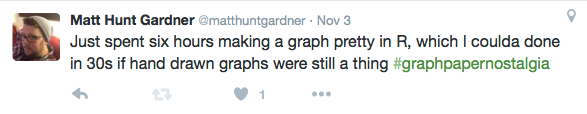
\includegraphics{images/tweet.png}

}

\caption{\label{fig-tweet}Actual tweet}

\end{figure}

\hypertarget{r-and-goldvarb}{%
\subsubsection{\texorpdfstring{\emph{R} and
\emph{Goldvarb}}{R and Goldvarb}}\label{r-and-goldvarb}}

In this guide I mention the program
\href{http://individual.utoronto.ca/tagliamonte/goldvarb.html}{\emph{Goldvarb}}
a lot. This is a well-known and widely-used program for doing
multivariate analysis in the language variation and change literature.
If you are are unfamiliar with \emph{Goldvarb} you can learn more in
Sali Tagliamonte's (2006)
\href{https://doi.org/10.1017/CBO9780511801624}{\emph{Analysing
Sociolingusitic Variation}}. I remain agnostic as to whether \emph{R} or
\emph{Goldvarb} or any other analysis tool is the one you must use for
your research. Each tool has pros and cons. These instructions are
simply a set of procedures you can use if you choose to use \emph{R}.

\hypertarget{token-files}{%
\subsubsection{Token Files}\label{token-files}}

You should have one master Microsoft \emph{Excel} spreadsheet for your
data. From this master spreadsheet you can create other files that can
be used in programs like \emph{Goldvarb} and \emph{R}. Each row of your
spreadsheet should represent an individual token. Each column of your
spreadsheet should represent a different, independent variable. The
example token file for this guide is structured this way, as in
Figure~\ref{fig-excel}.

\begin{figure}

{\centering 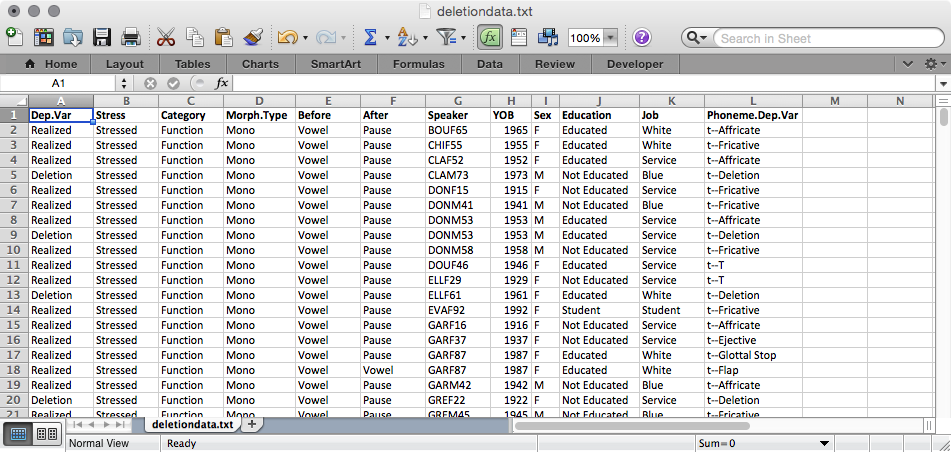
\includegraphics{images/tokenfile.png}

}

\caption{\label{fig-excel}Example token file \texttt{deletiondata.txt}}

\end{figure}

\begin{tcolorbox}[enhanced jigsaw, coltitle=black, colframe=quarto-callout-warning-color-frame, leftrule=.75mm, bottomtitle=1mm, arc=.35mm, opacitybacktitle=0.6, title=\textcolor{quarto-callout-warning-color}{\faExclamationTriangle}\hspace{0.5em}{Warning}, colbacktitle=quarto-callout-warning-color!10!white, breakable, left=2mm, titlerule=0mm, colback=white, toptitle=1mm, rightrule=.15mm, bottomrule=.15mm, toprule=.15mm, opacityback=0]
Do not include anything in your token file that isn't a token. Do not
create sum columns. Do not add random notes to the right or the top of
the data. \emph{R} will try to interpret all of this as data.
\end{tcolorbox}

\hypertarget{r-script-files}{%
\subsubsection{\texorpdfstring{\emph{R} Script
Files}{R Script Files}}\label{r-script-files}}

Anytime you are using \emph{R} you should be using script files. Script
files are very similar to \emph{Goldvarb} condition files. They are
files that include instructions that tell \emph{R} what to do. By saving
your command functions in script files you create replicability for your
work in \emph{R}. You may have \emph{pseudo}-script files already. Many
people keep a text file full of useful \emph{R} command functions. An
\emph{R} script file is an \emph{R}-specific file that does the same
thing.

I cannot stress enough the importance of replicability. You always want
to be able to go back and see every step you took in your analysis. This
is especially true in the frequent situation where a reviewer suggests
you go back and double-check something in your data or tweak your
analysis in some way. Using script files, which are essentially a log of
all your steps, is an excellent way to ensure replicability.

\begin{figure}

{\centering 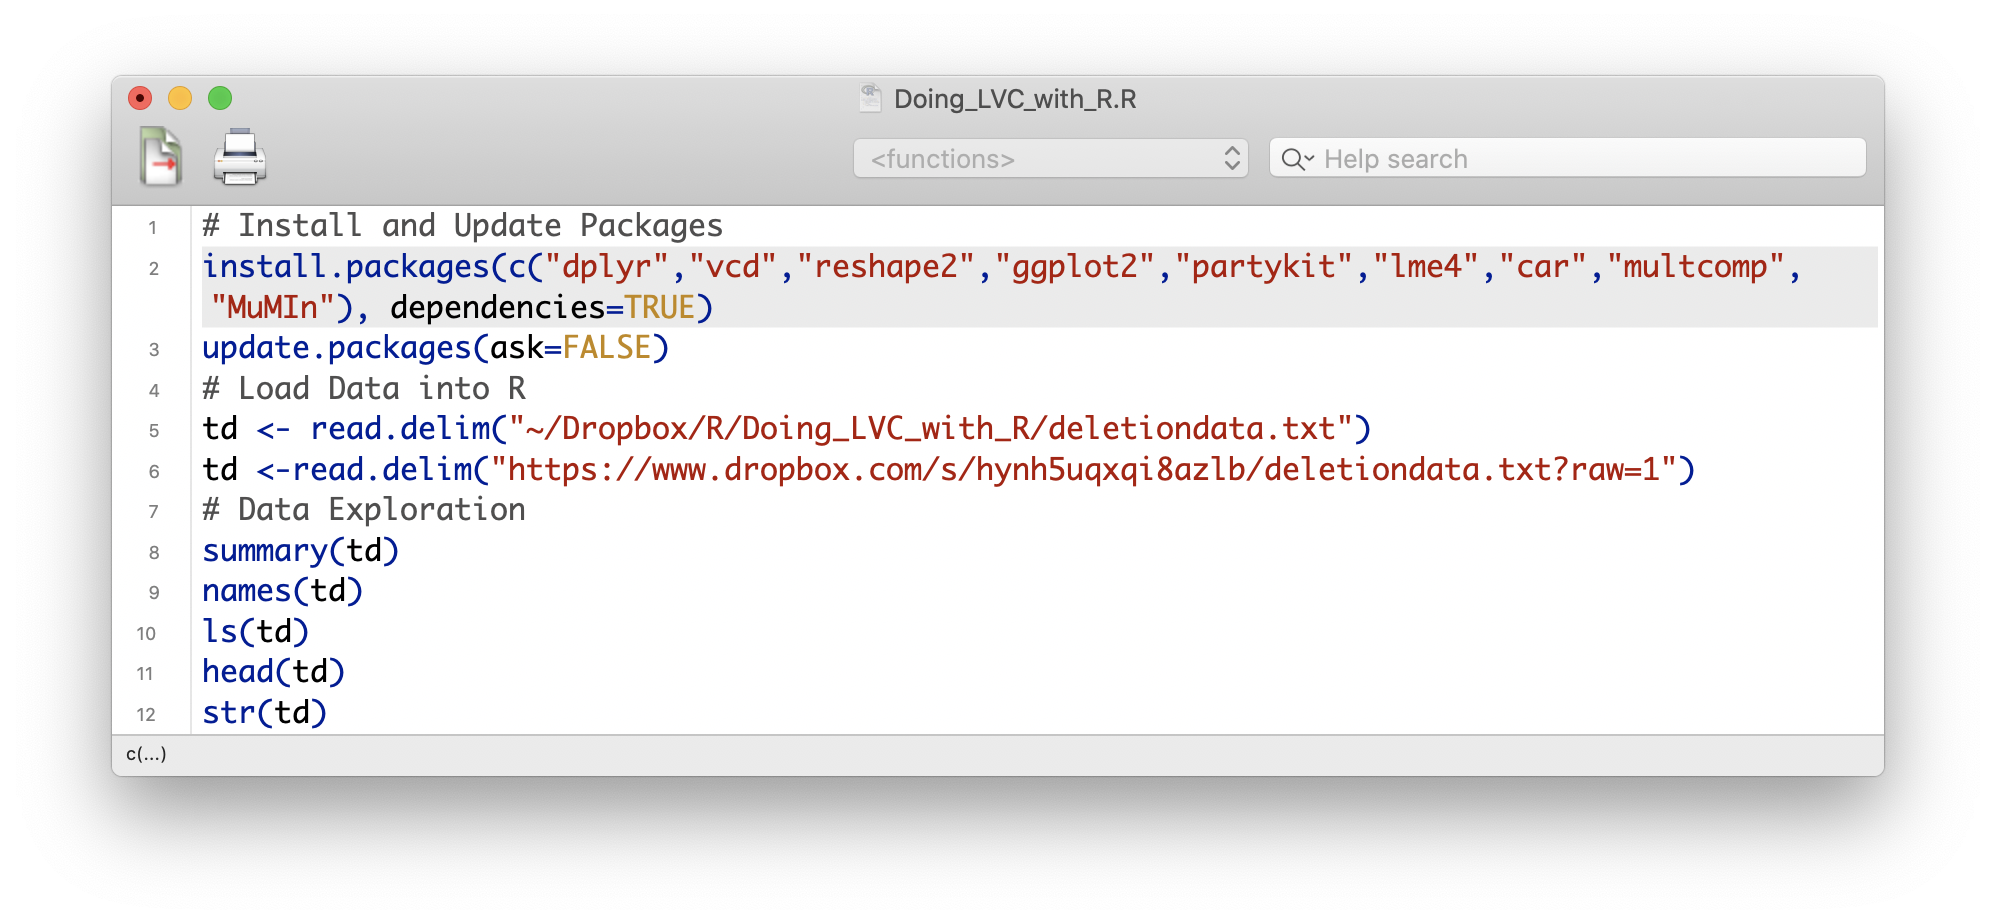
\includegraphics{images/scriptfile.png}

}

\caption{\label{fig-scriptfile}Example \emph{R} script file}

\end{figure}

Some people have one script file for an entire project --- say, a paper.
My co-author Derek Denis does this. Other people have specific script
files for specific results --- e.g., one script file for each graph with
the complete instructions for making that one graph, and the script file
and the graph it creates labelled identically. This is the method I
prefer. You may choose to do either, or both, or choose not to use
script files at all. It's up to you.

All of the functions discussed in this guide are in a single \emph{R}
script file which is replicated at the end of this guide.

If you download this file and open it, \emph{R} will automatically open
for you. If you want to create a new \emph{R} script file after you've
opened \emph{R} you can do so via the \textbf{File} menu:
\textbf{File\textgreater New Document}.

\hypertarget{r-and-r-studio}{%
\subsubsection{\texorpdfstring{\emph{R} and \emph{R
Studio}}{R and R Studio}}\label{r-and-r-studio}}

The following instructions assume you are using the core \emph{R}
program, not \emph{R Studio}. There is no real difference between these
programs (at least in how \emph{R} operates). \emph{R Studio} is just an
alternative user interface. Some of the external commands (e.g.~creating
a new \emph{R} script file, etc.) may be different, but the actual
\emph{R} functions listed in this document will be the same. There is no
advantage to using the \emph{R} core program or \emph{R Studio}. The
choice is simply personal preference. I prefer the core \emph{R} program
because I like to be able to see multiple script files at the same time.
\emph{R Studio} organizes script files in tabs. You may prefer \emph{R
Studio} because it can also author other types of documents.

To execute a command function that is in a script file simply put your
cursor on the same line as that command and press the execution or
\textbf{Run} command depending on your operating system and editor. In
Figure~\ref{fig-scriptfile} the cursor is placed in the middle of line
2; pressing \texttt{Control+Return} on my Mac executes the command
function highlighted in grey. You can also highlight a large portion, or
even all of your script file, and press the execution command to execute
multiple commands at once. There is also an execute all or
\textbf{Source} command that will execute the entire script file.

\hypertarget{tbl-execute}{}
\begin{longtable}[]{@{}lll@{}}
\caption{\label{tbl-execute}Execute current line of code}\tabularnewline
\toprule()
Execute & Mac OSX & Windows PC \\
\midrule()
\endfirsthead
\toprule()
Execute & Mac OSX & Windows PC \\
\midrule()
\endhead
\emph{R} Editor & \texttt{Command+Return} & \texttt{CTRL+R} \\
\emph{R Studio} & \texttt{Command+Return} & \texttt{CTRL+Enter} \\
\bottomrule()
\end{longtable}

\hypertarget{tbl-executeall}{}
\begin{longtable}[]{@{}lll@{}}
\caption{\label{tbl-executeall}Execute all code}\tabularnewline
\toprule()
Execute & Mac OSX & Windows PC \\
\midrule()
\endfirsthead
\toprule()
Execute & Mac OSX & Windows PC \\
\midrule()
\endhead
\emph{R} Editor & \texttt{Command+E} & \texttt{CTRL+Shift+R} \\
\emph{R Studio} & \texttt{Command+Option+R} & \texttt{CTRL+Alt+R} \\
\bottomrule()
\end{longtable}

\hypertarget{installing-packages}{%
\subsubsection{Installing Packages}\label{installing-packages}}

Before you begin doing any kind of analysis in \emph{R}, you'll first
need several `packages.' Packages are simply additional sets of
instructions that can do things above and beyond \emph{R}'s core
functionality. Packages are created by academics and are made available
to everyone. \emph{R} doesn't automatically download every package, so
if you want to use a specific package, you must download it. You only
need to do this one time. You also need to be connected to the internet
to do it. Type the following function into \emph{R}'s console window and
press \textbf{Enter/Return} or type it into a script file and press
\textbf{CTRL+Enter/Command+Return}:

\begin{Shaded}
\begin{Highlighting}[]
\FunctionTok{install.packages}\NormalTok{(}\FunctionTok{c}\NormalTok{(}\StringTok{"dplyr"}\NormalTok{, }\StringTok{"vcd"}\NormalTok{, }\StringTok{"reshape2"}\NormalTok{, }\StringTok{"ggplot2"}\NormalTok{,}
    \StringTok{"partykit"}\NormalTok{, }\StringTok{"lme4"}\NormalTok{, }\StringTok{"car"}\NormalTok{, }\StringTok{"multcomp"}\NormalTok{, }\StringTok{"MuMIn"}\NormalTok{,}
    \StringTok{"gmodels"}\NormalTok{), }\AttributeTok{dependencies =} \ConstantTok{TRUE}\NormalTok{)}
\end{Highlighting}
\end{Shaded}

Above \texttt{install.packages()} is a function for installing packages.
Inside the parentheses you tell \emph{R} which packages to install. In
this case you want to install multiple packages. Any time you need to
combine multiple things in \emph{R} you use the concatenating function
\texttt{c()}. So the above function says combine the package names
\texttt{dplyr}, \texttt{vcd}, \texttt{reshape2}, \texttt{ggplot2},
\texttt{partykit}, \texttt{lme4}, \texttt{car}, \texttt{multcomp}, and
\texttt{MuNIn} and then install the packages with those names. The
\texttt{dependencies\ =\ TRUE} specification tells \emph{R} to install
any additional packages that these packages depend on to function.

When you execute this function, \emph{R} might ask you to pick a
\textbf{CRAN Mirror}. This is just \emph{R} asking you from where you
want to download the packages. \emph{CRAN} is the \emph{Comprehensive R
Archive Network} and mirrors are simply different institutions that
offer identical copies of \emph{R} files for downloading. Usually I just
pick the option closest to me, which is the University of Toronto in
Canada. If you've downloaded packages in the past you've likely already
set your \textbf{CRAN Mirror}, and won't be prompted to do it again.

Once you've selected your \textbf{CRAN Mirror}, if necessary, and
executed the \texttt{install.packages()} function, you may see a bunch
of text scroll across your \emph{R} console window. This is just
\emph{R} telling you that it is downloading and installing these
packages. You can also install packages by selecting \textbf{Packages \&
Data \textgreater{} Package Installer}. In this window click \textbf{Get
List}, then search/browse for the required packages one by one. When you
find a package, highlight it and click \textbf{Install Selected}. Make
sure the \textbf{Install Dependencies} option is checked.

As \emph{R} updates over time, so too must these packages. But packages
don't update automatically. Therefore it's a good idea to periodically
execute the function below. Do this now. These instructions assume that
you have the most up to date version of \emph{R} and its packages. The
\texttt{ask=FALSE} option for the \texttt{update.packages()} function
just means that \emph{R} will run the update 'silently'', or rather, it
won't ask you whether or not you want to update each individual package
you've installed.

\begin{Shaded}
\begin{Highlighting}[]
\FunctionTok{update.packages}\NormalTok{(}\AttributeTok{ask =} \ConstantTok{FALSE}\NormalTok{)}
\end{Highlighting}
\end{Shaded}




\end{document}
